\clearpage
\section{Cross-validated sliding-windows}\label{sec:cross-validated-sw}
%%%%%

\info[inline]{Paragraph: Discuss other proposals for determining the optimal window length.}
Attempts have been made to improve \gls{sw} estimates by automatically extracting the optimal window length for a given scan from the data itself or to circumvent this issue~\parencite[see e.g.][]{Wang2014, Xu2015, Yaesoubi2018}.
In fact, prior work has established that knowing the optimal window length $w$ a priori can make \gls{sw} a remarkably effective method in the estimation of \gls{tvfc}~\parencite{Zalesky2015}.
These authors therefore argued that the window length should be set based on a rule of thumb after analyzing the \gls{bold} signal.
As such these can be considered \emph{data-driven} estimation methods as well.

\info[inline]{Paragraph: Introduce our way of cross-validating the optimal window length.}
Here we propose another data-driven way of determining the optimal window length: by using cross-validation.
Cross-validation is a simple yet effective technique to evaluate the generalizability performance of models~\parencite[see e.g.][section 8.2.4]{Deisenroth2019}.
In machine learning model development, it is often used to determine model hyperparameters.
%
In our approach, which we call the \gls{sw-cv} method, evaluation data points are taken from the middle of node time series.
For each of these data points individually, the likelihood of observing it under a zero-mean multivariate Gaussian for the full range of reasonable window lengths applied on all surrounding data points is taken (\emph{not} including the evaluation observation).
An example results matrix from this approach is shown in \cref{fig:sw-cv-demo}.
%
All proposal window lengths are odd numbers to ensure symmetry around the evaluation point.
The optimal window length $\hat{w}$ is then considered as the one where the average log likelihood over all evaluation data points is the highest:
\begin{equation}
  \hat{w} = \underset{w}{\arg\max} \frac{1}{N_e} \sum_{n}^{N_e} \left[ - \frac{D}{2} \log 2\pi - \frac{1}{2} \log | \hat{\mathbf{\Sigma}}_n | - \frac{1}{2} \mathbf{y}_n^T \hat{\mathbf{\Sigma}}_n^{-1} \mathbf{y}_n \right],
\end{equation}
where $1 \leq n \leq N_e$ is the evaluation data point, $N_e$ denotes the number of evaluation points (given by the total number of time steps~$N$ minus the maximum proposal window length~$w_{max}$), and $\hat{\mathbf{\Sigma}}_n$ (a function of $w$) is the (unbiased) covariance matrix estimate for all data points (excluding the evaluation data point) in the surrounding window of length~$w$.

As demonstrated in \cref{fig:sw-cv-demo}, this (log) likelihood is largest for longer window lengths if the covariance structure is static.
On the other hand, for a fast-changing covariance structure this likelihood is largest for shorter window lengths, allowing for picking up fast-changing covariance structures.


\begin{figure}[t]
  \centering
  \subcaptionbox{Static structure\label{fig:sw-cv-demo-static-structure}}{
    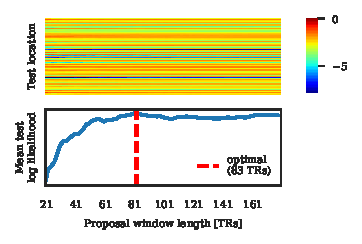
\includegraphics[width=0.47\textwidth]{fig/studies/cross_validating_sliding_windows/sw_cv_results_df_null}
  }
  \subcaptionbox{Fast-changing structure\label{fig:sw-cv-demo-fast-changing-structure}}{
    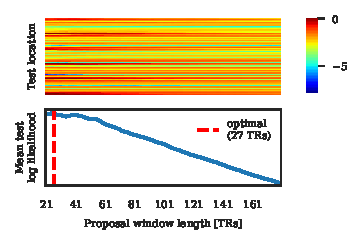
\includegraphics[width=0.47\textwidth]{fig/studies/cross_validating_sliding_windows/sw_cv_results_df_periodic_3}
  }
  \caption{
    Cross-validated sliding-windows demonstration showing how the optimal window length adapts to the underlying covariance structure.
    Heatmap colormaps indicate test location log likelihoods.
    Line plots show the mean test log likelihood over all test locations.
  }\label{fig:sw-cv-demo}
\end{figure}


\info[inline]{Paragraph: Discuss our particular implementation.}
The minimum and maximum window exploration lengths are set based on theoretical insights gathered over the past decade.
We leverage the existing wisdom in the field to choose $w_{min}$ and $w_{max}$ as 20~\parencite{Leonardi2015} and 180 seconds.
These are rounded up to the nearest odd number of \glspl{tr} to ensure symmetry.
%
The minimum window length ensures that we do not filter out signal in (expected) relevant frequency bands.
There is no actual constraint on maximum proposal window length limit.
If the signal is fundamentally static, we would expect the window length to trend to infinity.
However, doing so reduces the number of available evaluation points, so we are left with a trade-off.
%
After the optimal window length is determined, \gls{tvfc} estimates are generated in the same way as the regular \gls{sw} approach as discussed in \cref{subsec:sliding-windows-fc}.
%
Empirically, we show that this window length does indeed match the expected window length behavior on simulated data (see \cref{sec:simulations-results}).
